\documentclass[nonumbib,leqno]{nrc1} 
\usepackage{amssymb, amsmath, bm, epsfig,psfrag,graphicx}
\usepackage[french, english]{babel}
\usepackage{setspace}
\usepackage{lineno}
\usepackage{natbib}
\usepackage{longtable}
\usepackage{booktabs}
%added 9/29/08
%\usepackage[nolists]{endfloat}
\bibpunct{(}{)}{;}{a}{}{;}
\setlength{\mathindent}{1cm}

\setcounter{page}{1}
\volyear{XX}{201X}
\journal{Can. J. Fish. Aquat. Sci.}

\received{}

\bibliographystyle{ecology}

\begin{document}

\title{Assessing the detectability of prey removal effects on Stellar sea lion ({\it Eumetopias jubatus}) abundance}

\author[P. B. Conn, D. S. Johnson, L. W. Fritz, B. S. Fadely]{Paul B. Conn, Devin S. Johnson, Lowell W. Fritz, Brian S. Fadely}
\address{National Marine Mammal Laboratory, Alaska Fisheries Science Center,
NOAA National Marine Fisheries Service,
Seattle, Washington, U.S.A. 98115}
\correspond{paul.conn@noaa.gov}

\shortauthor{Conn et al.}
\large

\maketitle

{\sc Running Head}: Prey removal and Steller sea lions \bigskip

May 13, 2013



\clearpage

\linenumbers

%% ABSTRACT %%%%%%%%%%%%%%%%%%%%%%%%%%%%%%%%%%%%%%%%%%%%%%%%%%%%%

%{\sc Summary.}
\begin{abstract}
\large
we'll do this last
%\keywords{}
\end{abstract}

%\begin{resume}
%\end{resume}

\keywords{Stellar sea lions}


\clearpage

\renewcommand{\baselinestretch}{1.8}\normalsize


\section{Introduction}

1. Stellar sea lion status relative to ESA, Western vs Eastern stock, decline proportion (from trend reports?)

2. Mitigation measures affect fisheries, lack of consensus on proximate causes of decline

3. Data at hand to assess relationship between fishing and Stellar sea lion demography: adult \& pup,
A large number of studies have been conducted attempting to relate Stellar sea lion abundance (pup counts, non-pup counts, `growth rate') to fishery variables (catch, No. hauls, CPUE [catch per tow]).  Results of these studies. Reasons why these data aren't ideal.  Inferences made from lack of significant results (i.e. Bernard et al. want to infer lack of relationship from lack of significant tests).



In this paper, we use simulation to investigate whether available SSL aerial survey metrics (adult or pup counts, count ratios) and explanatory variables commonly compiled from fisheries datasets are sufficient to reveal relationships between SSL population dynamics and prey availability. To conduct simulations, we consider the joint dynamics of SSL, a prey population, and a fishery.  A tacit assumption in all of our simulations is that sea lion dynamics depend on availability of the prey resource through one or more demographic component (e.g. fecundity, survival).  Due to data limitations and the complexity of simulated dynamics, our approach makes a number of simplifying assumptions (e.g. spatially independent populations, a single prey species).  However, these simplifications all serve to increase the power of detecting a relationship between fishing and SSL abundance; if we cannot do a good job of relating the two with simulated data, our case is even more hopeless in the real world!

The remainder of this article is structured as follows.  First, we describe a number of alternative models for the coupled fishery and SSL dynamics.  These models are intended to encompass a number of
alternative states of nature, including the functional relationship between sea lions and fish, as well as
how fishing effort is allocated (i.e., whether or not it is dependent on fish distribution).  Next, we provide details on how we calibrated these models to generate reasonable parameter estimates for simulation.  We then describe our overall simulation structure and provide details on the simulation outputs (e.g., conventional test statistics, Bayesian model weights) that we used to measure our ability to detect relationships between SSL abundance and explanatory fisheries variables.  After describing results, we conclude by offering some final thoughts about how best to interpret SSL-fisheries interactions on the base of available data.


\section{Methods}

We considered models for coupled dynamics between fishers, fish, and SSL, where fish and SSL were modeled as island populations (i.e. assuming independent dynamics among islands).  In reality, there are substantial dispersal of SSL among rookery and haulout areas.  Similarly, relevant fish populations in the Gulf of Alaska and Bering Sea (e.g., Atka mackerel, pacific cod, walleye pollock) are interconnected through movement and recruitment processes.  However, the assumption of independent dynamics should provide greater power for detecting meaningful relationships between SSL aerial survey counts and fishery variables since responses of SSL to experimental treatments (fishing) are not blurred by uncontrollable and poorly understood processes.  Thus, a simulation design assuming island populations should provide a useful one-way test for whether the approach of relating fishery variables to SSL counts provides reasonable inferences.

\subsection{Models}


To induce coupled dynamics between SSL, fish, and fishers, we modeled
fish mortality as a function of both fishing effort and SSL predation, where annual fish recruitment follows a Beverton-Holt spawner-recruit function \citep{BevertonHolt1957} with lognormal error (separate models for state dynamics are modeled for each island population).  In turn, we made SSL dynamics dependent on the expected per capita number of fish ``harvested" by SSL, where dependency can be expressed in terms of survival or fecundity (depending upon simulation configuration).  Finally, we considered two scenarios for fisher dynamics, allowing fishing effort to be (i) randomly allocated each year, or (ii) allocated in proportion to fish biomass in each island population.  Each of these components are described in further detail below.


\subsubsection{Stellar sea lion model}

We based SSL dynamics loosely on the age-structured (`HFYS') Leslie-matrix model described by \citet{HolmesEtAl2007}, who summarized female fecundity and survival probability for SSL for ages $0-30$ (survival probability was assumed zero after age 30).  This model assumes a post-breeding census, coinciding with annual aerial surveys of rookeries and haul-outs in the Gulf of Alaska and Aleutian islands in June and July.  As presented, this `base' Leslie-matrix has a dominant eigenvalue of 1.0014, which is indicative of a stable population (at least in absence of demographic stochasticity).

To make SSL demography dependent on the number of fish, we allowed either fecundity at age ($f_{a,t,k}$) or survival at age ($S_{a,t,k}$) (Table \ref{tab:model}) to be dependent on the ratio of fish to sea lion biomass.  As each of these parameters is bounded in the $(0,1)$ interval, we included simple formulations where
\begin{linenomath}
\begin{equation*}
{\rm logit}(S_{a,t,k})=\alpha_{0,a} + \alpha_1 B_{t,k}^*/B_{t,k} \hspace{2mm} {\rm or}
\end{equation*}
\end{linenomath}
\begin{linenomath}
\begin{equation*}
{\rm logit}(f_{a,t,k})=\beta_{0,a} + \beta_1 B_{t,k}^*/B_{t,k}.
\end{equation*}
\end{linenomath}
Here, $S_{a,t,k}$ gives survival of age $a$ SSL in year $t$ of simulation for site $k$, $f_{a,t,k}$ gives SSL fecundity for age $a$ in year $t$ and site $k$, $B_{t,k}^*$ gives SSL biomass in year $t$ in site $k$, and $B_{t,k}$ gives fish biomass in year $t$ and site $k$ (for a complete list of notation, see Table \ref{tab:model}).  We calibrate parameters describing the hypothetical relationship between demographic parameters and relative biomass of SSL and prey at the start of year $t$ ($\alpha_0,\alpha_1,\beta_0,\beta_1$) to produce reasonable time series in a later section (see \ref{section:Calibration}).

\subsubsection{Prey (fish) model}

A variety of commercially important fish stocks are affected by time-area closures designed to protect SSL, most notably walleye pollock ({\it Theragra chalcogramma}), pacific cod ({\it Gadus macrocephalus}), and Atka mackerel ({\it Pleurogrammus monopterygius}).  Rather than base fish dynamics on just one (or multiple) of these species, we modeled fish dynamics of a hypothetical, generic species that combined similar life history and exploitation features from each stock.  For simplicity, we use the same annual time step for the fish population as for SSL, modeling recruitment as occurring immediately prior to annual aerial surveys.  An age-structured population dynamics model was assumed for each simulated fish stock, with 10 ages (1-9 and 10+).
We write total mortality rate for a given fish age class $a$ at time $t$ at site $k$ as $Z_{a,t,k}=M + F_{t,k}^* + F_{a,t,k}$, where $M$ gives
natural mortality, $F_{t,k}^*$ gives a mortality rate attributable to SSL in site $k$ in year $t$ of simulation, and $F_{a,t,k}$ gives time- and age-specific fishing morality (recall that notation is also defined in Table \ref{tab:model}).  Recent assessments of walleye pollock, pacific cod, and Atka mackerel stocks \citep[e.g.][]{PollockAssessment2011,PacCodAssessment2011,AtkaAssessment2012} indicated natural mortality rates in the 0.3-0.34 range.  However, these figures include all natural mortality, including SSL predation (which we model separately).  For our hypothetical fish stock, we set $M=0.2$ during simulations.

We had little information on age- or size-selectivity of target species by SSL, so considered all fish age classes as fully selected by SSL predation.  By contrast, we modeled fishing mortality, $F_{a,t,k}$, as a product of an age-specific selectivity curve and a fully selected fishing mortality rate that is itself a function of fishing effort, such that $F_{a,t,k}=q E_{t,k} s_a$, where $E_{t,k}$ summarizes fishing effort for site $k$ in year $t$, $s_a$ describes selectivity at age, and $q$ is a catchability coefficient.  Recent assessments of fish stocks in the Bering sea used flexible selectivity functions that were allowed to evolve over time; these pointed to dome-shaped selectivity functions in the majority of cases.  For simulations, we used a dome-shaped double logistic model constructed so as to approximate the general shape obtained in the assessments (Fig. \ref{fig:at_age}, Table \ref{tab:model}).  For further description of effort and catchability, we refer the reader to subsequent sections \ref{section:Fleet} and \ref{section:Calibration}, respectively.

For SSL-related mortality, we imposed a model of the form $F_{t,k}^*=\delta N_{t,k} B_{t,k}^*$, where $N_{t,k}$ gives the total number of fish in population $k$ at time $t$, $B_{t,k}^*$ gives the SSL biomass at time $t$, and $\delta$ gives a capture efficiency parameter. This is a similar functional form as used in classic Lotka-Volterra predator-prey models \citep[see e.g.][]{Gotelli2001}, with the modification that we use biomass (instead of numbers) of SSL to allow for the fact that larger sea lions will likely consume more fish than smaller ones.  Once again, we leave it until a later section (\ref{section:Calibration}) to determine reasonable values for $\delta$.

Annual recruitment at each site was modeled using a Beverton-Holt spawner-recruit curve subject to lognormal error.  A modern parameterization of this model is
\begin{linenomath}
\begin{equation*}
N_{1,t+1,k} = \frac{0.8 R_{0,k} h SSB_{a,t,k}}{0.2 \phi_0 R_{0,k}(1-h)+(h-0.2)SSB_{t,k}} \exp{\epsilon_{t,k}},
\end{equation*}
\end{linenomath}
where $N_{1,t,k}$ gives the number of recruits (age 1 individuals) in year $t$ at site $k$, $R_{0,k}$ is expected annual recruitment in absence of fishing (allowed to be different across sites), $SSB_{t,k}$ gives spawning biomass in year $t$, $h$ is steepness, $\phi_0$ is unfished spawning biomass per recruit (calculated in absence of SSL), and $\epsilon_{t,k}$ represents Gaussian noise \citep{MaceDoonan1988}.  Spawning stock biomass can be calculated from knowledge of numbers of fish in each age class, together with maturity at age and weight at age vectors (Table \ref{tab:model}).

\subsubsection{Fleet dynamics}
\label{section:Fleet}

We considered two scenarios for fleet dynamics, both of which assume that total fishing effort stays constant
over the course of simulation time (at least in portions of simulation time series where fishing occurs).  In the first scenario, we allow fishing effort to be annually redistributed according to a ${\rm Dirichlet}(1,1,\hdots,1)$ distribution.  This formulation approximates the situation where experimental treatments (fishing) are applied randomly to experimental units (sites).  As such it is clearly unrealistic, as fishing vessels will likely try to optimize catch by going to areas where there are more fish, perhaps subject
to economic and time constraints (e.g., distances from port).  Nevertheless, this scenario likely provides the greatest power to detect relationships between SSL survey counts and fishing variables.

Our second scenario assumes that fishing fleets redistribute effort each year according to the relative number of fish at each site.  This scenario is also clearly unrealistic, as it assumes fishers have omniscient knowledge about the distribution and abundance of fish, and no economic constraints influencing their movements (e.g. fuel costs, time).  However, this distribution of effort represents an ideal free distribution \citep{FretwellLucas1970}, which has a rich use in ecology.  It also represents the opposite end of the spectrum from the first scenario, where there was no relationship between fishing effort and fish abundance.

For each scenario, we calculated catch at each site using the Baranov catch equation \citep{Baranov1918}:


\subsubsection{Survey models/measurement error}

We investigate the case where $K=?$ sites are surveyed by annual SSL aerial surveys that count the total
number of adults (age 2+) each year.  Aerial survey counts are an imperfect measure of abundance for two reasons.  First, not all animals are present on haul-outs or rookeries when surveys are conducted, because some proportion are out foraging.  Second, survey counts are subject to measurement error (not all animals present are counted).  \citet{HolmesEtAl2007} investigated the variability of counts from repeat aerial surveys that were conducted in the same year, and suggested that the coefficient of variation (CV) for these counts was $\approx 5\%$.  We used this value to induce measurement error on observed counts, assuming that 
\begin{linenomath}
  \begin{equation}
     I_{t,k} \sim {\rm Normal}(N_{2+,t,k}^*,[0.05 N_{2+,t,k}^*]^2),
  \end{equation}
\end{linenomath}
where $I_{t,k}$ gives the adult survey count at site $k$ at time $t$ and $N_{2+,t,k}^*=\sum_{a=2}^30 N_{a,t,k}^*$ (in practice, we rounded $I_{t,k}$ to the closest integer after simulation measurement error).  We acknowledge that the small CV of 0.05 understates likely variation in the relationship between survey counts and underlying abundance; for instance, the portion of animals available for sampling each year may change if the time spent foraging changes (e.g., in responses to prey abundance).  Nevertheless, our approach is consistent with the goal of maximizing power to detect prey removal effects on SSL abundance.

Also investigate a pup scenario?

\subsection{Simulation design}

We utilized a $2 \times 2$ factorial simulation design that included design points for each combination of fleet effort allocation (random or proportional to fish abundance) and SSL demographic component (whether fecundity or survival was related to prey availability).  For each design point, we conducted 1000 simulations, each of which had a similar overall design (Fig. \ref{fig:sim_diagram}).  
In each simulation, we randomly generated virgin fish recruitment ($R_{0,k}$) at each of $xx$ sites, and initialized prey and SSL abundance according to their stable age distributions \citep[cf.][]{Caswell2001}, assuming an initial abundance of 600 SSL at each site.  We then simulated dynamics of SSL and prey for 100 years in absence of fishing, a time period which allowed SSL abundance to stabilize with the number of prey available.  This approach also induced stochasticity in the age structure of both species (resulting from annual fish recruitment variation).  We then introduced fishing, and aerial surveys were simulated beginning 10 years later (these were conducted for the next 35 years of simulation time).  These time periods were selected to approximate the introduction of fishing pressure and the institution of aerial SSL surveys in the Bering Sea and Gulf of Alaska; for relevant fish stocks (e.g. Alaska pollock), heavy commercial fishing began to ramp up in the mid-late 1960s, with aerial surveys beginning in 1976.  The survey collection period of 35 years approximates data collection up through 2010.  For each simulation, we also used the time series of simulated recruitment deviations to calculate what SSL abundance would have been at the end of simulation time if there had been no fishing (i.e., if $F_{a,t,k}=0$).

Following each simulation, we attempted to test whether SSL counts ($I_{t,k}$) were related to fishing variables ($C_{t,k}$,$L_{t,k}$,$U_{t,k}$) by fitting generalized estimating equations (GEE) to the data, where the response variable ($I_{t,k}$) was modeled using a Poisson error structure.  The GEE approach to data analysis was developed for analysis of longitudinal data \citep{LiangZeger1986}, where responses of individual subjects are possibly dependent (GEEs still assume that individual's responses are independent).  This formulation is a natural approach for the analysis of SSL survey counts, as ``responses" across years but within sites are autocorrelated.  In particular, we fit models where the expected count at site $k$ was modeled according to
\begin{linenomath}
  \begin{equation*}
     E(I_{t,k})=\gamma_{0,k} + \gamma_1 X_{t,k},
  \end{equation*}
\end{linenomath}
where $\gamma_{0,k}$ gives a site-specific intercept term, $\gamma_1$ is a slope parameter, and $X_{t,k}$ is a fishery variable used for prediction.  We fit three such models to each dataset, including (1) $X_k = C_{t,k}$, (2) $X_k = L_{t,k}$, and (3) $X_k=U_{t,k}$.  We used an AR1 correlation structure for each model (i.e. assuming that observations within a particular site were autocorrelated). After fitting this model using the \texttt{gee} package in R, we used the robust $Z$-statistic output for $\gamma_1$ to determine whether the fishery variable $X_{t,k}$ was (a) positively related to SSL counts ($Z>1.96$), (b) negatively related to SSL counts ($Z<1.96$), or (c) whether the null hypothesis of no relationship could not be rejected at the $\alpha=0.05$ level ($-1.96<Z<1.96$).

Analyze trend too? (i.e. use $I_{t,k}/I_{t-1,k}$)?

\subsection{Calibration}
\label{section:Calibration}

Several simulation inputs (Table \ref{tab:inputs}) required a calibration exercise to determine reasonable values prior to simulation.  These included parameters describing SSL fecundity as a function of prey availability ($\alpha_0$ and $\alpha_1$), those describing SSL survival as a function of prey availability ($\beta_0$ and $\beta_1$), capture efficiency of SSL ($\delta$), and fish catchability associated with fishing effort ($q$).

General approach $\rightarrow$ Use simulated annealing to minimize an objective function penalizing
deviations from the following: (SSL lambda = 1 prior to fishing, observed SSL population decline, F in current year for fishery = 0.3, F for SSL = 0.1).


\section{Results}

\section{Discussion}

To date, the most comprehensive analyses addressing SSL declines have largely implicated decreases in recruitment as a likely reason for non-recovery of the western stock.  For instance, \citet{HolmesEtAl} estimated the life history components that would need to be reduced to result in
the patterns of observed population decline exhibited in SSL datasets from 1976-2004.  They found support for a model with a sudden, albeit temporary drop in non-pup survival in the early 1980s coupled with an overall decrease in birth rates.  This finding implicates reduced non-pup survival in the initial crash of SSL; however, chronic depression in birth rates appears to be the primary reason why SSL stocks have not recovered.  Similarly, \citet{WolfeMangel2008} fit alternative models encompassing several different working hypotheses about SSL decline, and found strong support for models where pup recruitment was written as a function of total prey availability or prey species composition.

\bibliography{SSLfish_biblio}

\begin{longtable}{p{4cm}lll p{8cm}}
\caption[Population \& Fisheries dynamics]{\large Notation and dynamical equations used to simulate
 hypothetical Stellar sea lion (SSL), fish, and fisheries data.} \label{tab:model} \\
%\begin{tabular}{p{4cm}lll p{8cm}}
\hline \hline 
Quantity & & Symbol & & Description or definition \\
\cline{1-1} \cline{3-3} \cline{5-5} \\
\endfirsthead
\hline \hline
Quantity & & Symbol & & Description or definition \\
\cline{1-1} \cline{3-3} \cline{5-5} \\
\endhead
\hline
\endfoot
\hline
\endlastfoot
\multicolumn{1}{l}{\textbf{Stellar sea lion dynamics}}\\
Numbers at age & & $N_{a,t,k}^*$ & & Number of age $a$ SSL during surveys in year $t$ at site $k$\\
Biomass at age & & $B_{a,t,k}^*$ & & Biomass of age $a$ SSL during surveys in year $t$ at site $k$\\
Total biomass & & $B_{t,k}^*$ & & Total SSL biomass at site $k$ during surveys in year $t$ ($B_{t,k}^*=\sum_a B_{a,t,k}$) \\
Annual survival & & $S_{a,t,k}$ & & Probability of age $a$ SSL survival from year $t$ to year $t+1$ at site $k$ \\
Fecundity & & $f_{a,t,k}$ & & Expected number of pups per age $a$ SSL female in year $t$ at site $k$ \\
Leslie matrix model & & ${\bf A}_{t,k}$ & & Leslie matrix model (composed of $S$ and $f$ values) for SSL dynamics \\
Abundance at age & & ${\bf N}_{t+1,k}$ & & ${\bf N}_{t+1,k}={\bf A}_{t,k} {\bf N}_{t,k}$, where \newline ${\bf N}_{t,k}$ is an abundance-at-age vector \\
\midrule
\multicolumn{1}{l}{\textbf{Fish dynamics}}\\
Weight-at-age & & $w_a$ & & $w_a = [ 1 + \exp(-b^{\rm wgt}(a-a_{50}^{wgt})) ]^{-1}$ \\
Maturity-at-age & & $m_a$ & & $m_a = [ 1 + \exp(-b^{\rm mat}(a-a_{50}^{mat})) ]^{-1}$ \\
Unfished spawning biomass per recruit & & $\phi_0$ & & $\phi_0=\sum_{a=1}^9 \{ \exp(-aM) w_a m_a \} + \frac{\exp(-10M) w_{10} m_{10}}{1-\exp(-M)}$ \\

Fishery selectivity  & & $s_a$ & &  $s_a = \frac{1}{1+\exp(-\eta_1(a-\kappa_1))} \left( 1- \frac{1}{1+\exp(-\eta_2(a-\kappa_2))} \right)$ (rescaled to have a maximum of 1.0)\\

Fishery mortality rate & & $F_{tk}$ & & $F_{tk}=q E_t$, Fully selected fishing mortality rate for year $t$, site $k$\\

Fishing mortality rate at age & & $F_{a,t,k}$ & & $F_{a,t,k}=s_a F_{t,k}$ \\

SSL predation rate  & & $F_{t,k}^*$ & & $F_{t,k}^*=\delta N_{t,k} B_{t,k}^*$ \\

Natural mortality rate & & $M$ & & Assumed constant (0.2) for all simulations \\

Total mortality rate at age & & $Z_{a,t,k}$ & & $Z_{a,t,k}=M+F_{a,t,k}+F_{a,t,k}^*$ \\[2pt]
\\

Abundance at age & & $N_{a,t,k}$ & & $N_{1,1,k} = R_{0,k}$ \newline
$N_{a+1,1,k}=N_{a,1,k}\exp(-Z_{a,1,k})~~~\forall a \in (1\ldots 9)$ \newline
$N_{10,1,k}=N_{9,1,k} \frac{\exp( -Z_{9,1,k})} {1-\exp (-Z_{10,1,k})}$ \newline
$N_{1,t+1,k}=\frac{0.8 R_{0,k} h SSB_{t,k}} {0.2\phi_0 R_{0,k} (1-h)+(h-0.2)SSB_{t,k}}
  \exp(\epsilon_{t,k}^R)$ \newline
$N_{a+1,t+1,k}=N_{a,t,k}\exp(-Z_{a,t,k})~~~\forall a \in (1\ldots 9)$ \newline
$N_{10,t,k}=N_{10,t-1,k} \frac{\exp( -Z_{9,t-1,k})}{1-\exp (-Z_{10,t-1,k})}$ \newline
where $\epsilon_{t,k}^R \sim {\rm Normal}(0,\sigma_R)$, $\phi_0$ gives unfished spawning biomass per recruit, and $h$ gives steepness (set to 0.8).  \\[2pt]

Total abundance by site & & $N_{t,k}$ & & $ \sum_a N_{a,t,k}$ \\

Spawning biomass & & $SSB_{t,k}$ & & $S_{t,k}=\sum_a N_{a,t,k} w_a m_a$ \\

\midrule

\multicolumn{1}{l}{\textbf{Fleet dynamics}}\\

Fishing effort (random) & & $E_{t,k} $ & & $ E_{t,k} \sim {\rm Dirichlet}(1,1,\hdots,1)$ \\[2pt]

Fishing effort (directed) & & $E_{t,k}$ & & $ E_{t,k} = B_{t,k}/\sum_{k} B_{t,k} $, \newline \\[2pt]

Catchability & & $q$ & & Relates fishing mortality rate to effort (see $F_{t,k}$ definition) \\

Catch-at-age & & $C_{a,t,k}$ & & Calculated with Baranov catch equation: $C_{a,t,k}=F_{a,t,k}/Z_{a,t,k} (1-\exp(-Z_{a,t,k}) N_{a,t,k}$ \\ 

Catch (numbers) & & $C_{t,k}$ & & $C_{t,k}=\sum_a C_{a,t,k}$ \\

Catch (weight) & & $L_{t,k}$ & & $L_{t,k}=\sum_a C_{a,t,k} w_a$ \\

CPUE Index & & $U_{t,k}$ & & $U_{t,k} \sim {\rm lognormal}(\log(L_{t,k}/E_k),\sigma^2)$, where $\sigma=\sqrt{log(0.2^2+1)}$ (implying a CV of 0.2) \\

\midrule

\multicolumn{1}{l}{\textbf{Aerial survey data}}  \\
Adult survey count  & & $I_{t,k}$ & & Count of adult (age 2+) SSL during the simulated aerial survey of site $k$ at time $t$\\
\bottomrule
%\end{tabular}
\end{longtable}

\begin{table}
\caption{\setstretch{2} \large Definitions and values for simulation input variables.  The subscript $\dag$
indicates values that were fixed as an outcome of calibration exercises; remaining simulation inputs were
set a priori.}
\label{tab:inputs}
\begin{tabular}{p{3cm}lll p{9cm}}
\\
\hline \hline
Input variable & & Range & & Definition\\
\cline{1-1} \cline{3-3} \cline{5-5}
\\
\multicolumn{1}{l}{\textbf{Survey variables}}  \\
$Y_1$ & & 100 & & Number of simulation years with just SSL (no fishing) \\
$Y_2$ & & 10 & & Number of years of fishing before aerial surveys begin \\
$Y_3$ & & 30 & & Number of years with both fishing and simulated aerial surveys \\
$K$ & & ??? & & Number of ``sites" (SSL populations)  \\
\midrule
\multicolumn{1}{l}{\textbf{SSL variables}}  \\
$p$ & & 0.8 & & SSL availability probability \\
$\alpha_{0,a}^\dag$ & & xx & & Intercept of SSL survival model (logit scale) \\
$\alpha_1^\dag$ & & xx & & Slope parameter of SSL survival model (logit scale); controls per capita dependence
                     on prey abundance \\
$\beta_{0,a}^\dag$ & & xx & & Intercept of SSL fecundity model (logit scale) \\
$\beta_1^\dag$ & & xx & & Slope parameter of SSL fecundity model (logit scale); controls per capita dependence
                    on prey abundance \\
$\delta^\dag$ & & xx & & Capture efficiency parameter describing the rate at which SSL/fish encounters result in fish mortality (such that $F_{t,k}^*=\delta N_{t,k} B_{t,k}^*$) \\
\midrule
\multicolumn{1}{l}{\textbf{Fish variables}}  \\
$M$ & & 0.2 & & Natural mortality rate (in absence of SSL) \\ [2pt]
$R_{0,k}$ & & U(100000,5000000) & & Virgin recruitment at site $k$; drawn from a uniform distribution at the beginning of each simulation \\
$h$ & & 0.8 & & Beverton-holt steepness \\
$\sigma_R$ & & 0.5 & & Standard deviation for lognormal recruitment deviations \\
$a_{50}^{\rm mat}$ & & 5 & & Age at 50\% sexual maturity \\
$b^{\rm mat}$ & & 1 & & Slope parameter for logistic maturity-at-age function \\
$a_{50}^{\rm wgt}$ & & 5 & & Age at 50\% weight \\
$b^{\rm wgt}$ & & 0.7 & & Slope parameter for logistic weight-at-age function \\
$\eta_1$ & & 1.3 & & Slope of ascending limb of double logistic selectivity curve \\
$\eta_2$ & & 1 & & Slope of descending limb of double logistic selectivity curve \\
$\kappa_1$ & & 4 & & Age at 50\% fishery selectivity (ascending) \\
$\kappa_2$ & & 10 & & Age at 50\% fishery selectivity (descending) \\
$\sigma_I$ & & 0.05 & & Coefficient of variation (CV) for aerial survey counts \\
$ q^\dag $ & & xxx & & Catchability coefficient relating fishery effort ($E_{a,t,k}$) to apical fishing mortality \\
\bottomrule
\end{tabular}
\vspace{4in}
\end{table}

\begin{figure}
\begin{center}
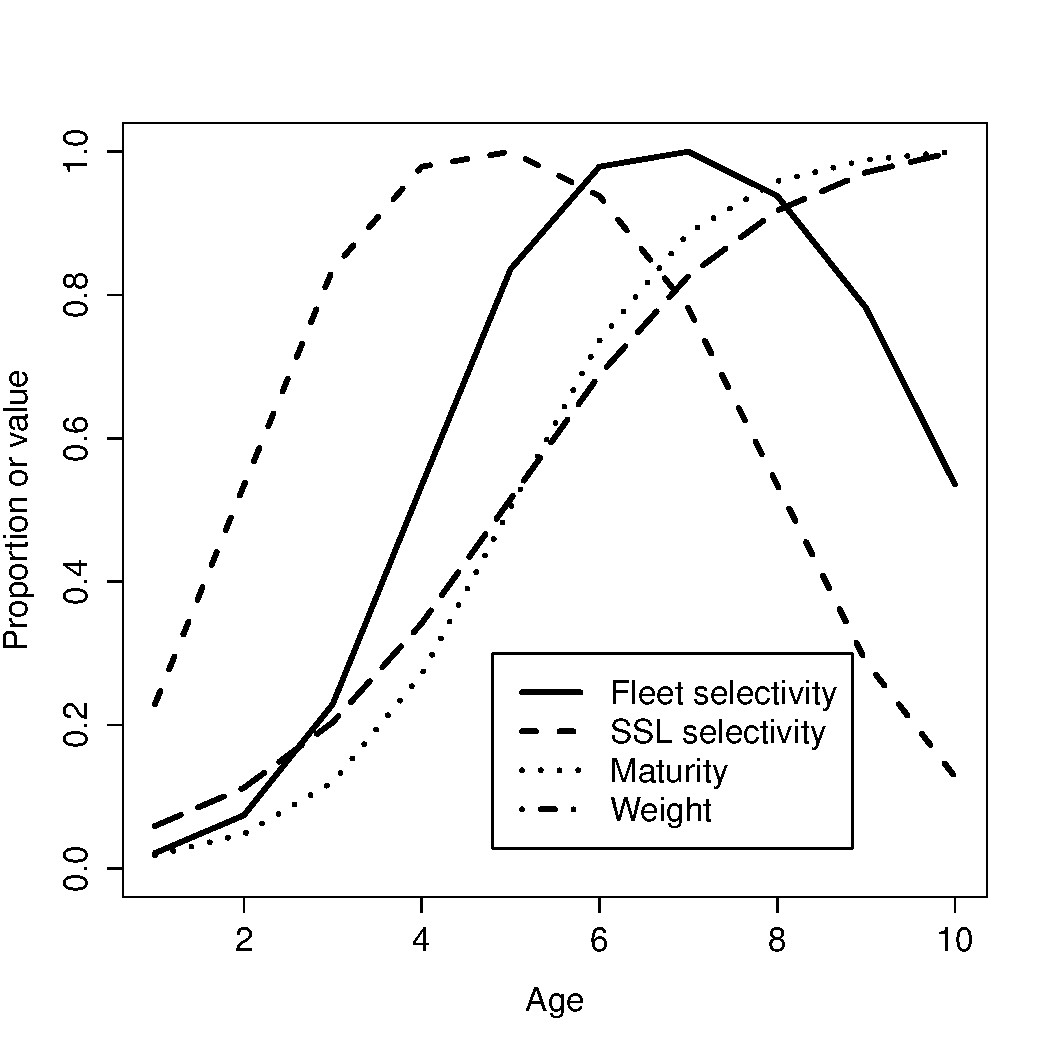
\includegraphics[width= \textwidth]{At_age_plots.pdf}
\end{center}
\caption{An illustration of fishery selectivity-at-age (`Selectivity'), proportion of fish sexually
mature by age (`Maturity'), and weight-at-age (`Weight'; standardized to have a maximum of 1.0) used
in SSL-fisheries simulation analyses.}
\label{fig:at_age}
\end{figure}

\begin{figure}
\begin{center}
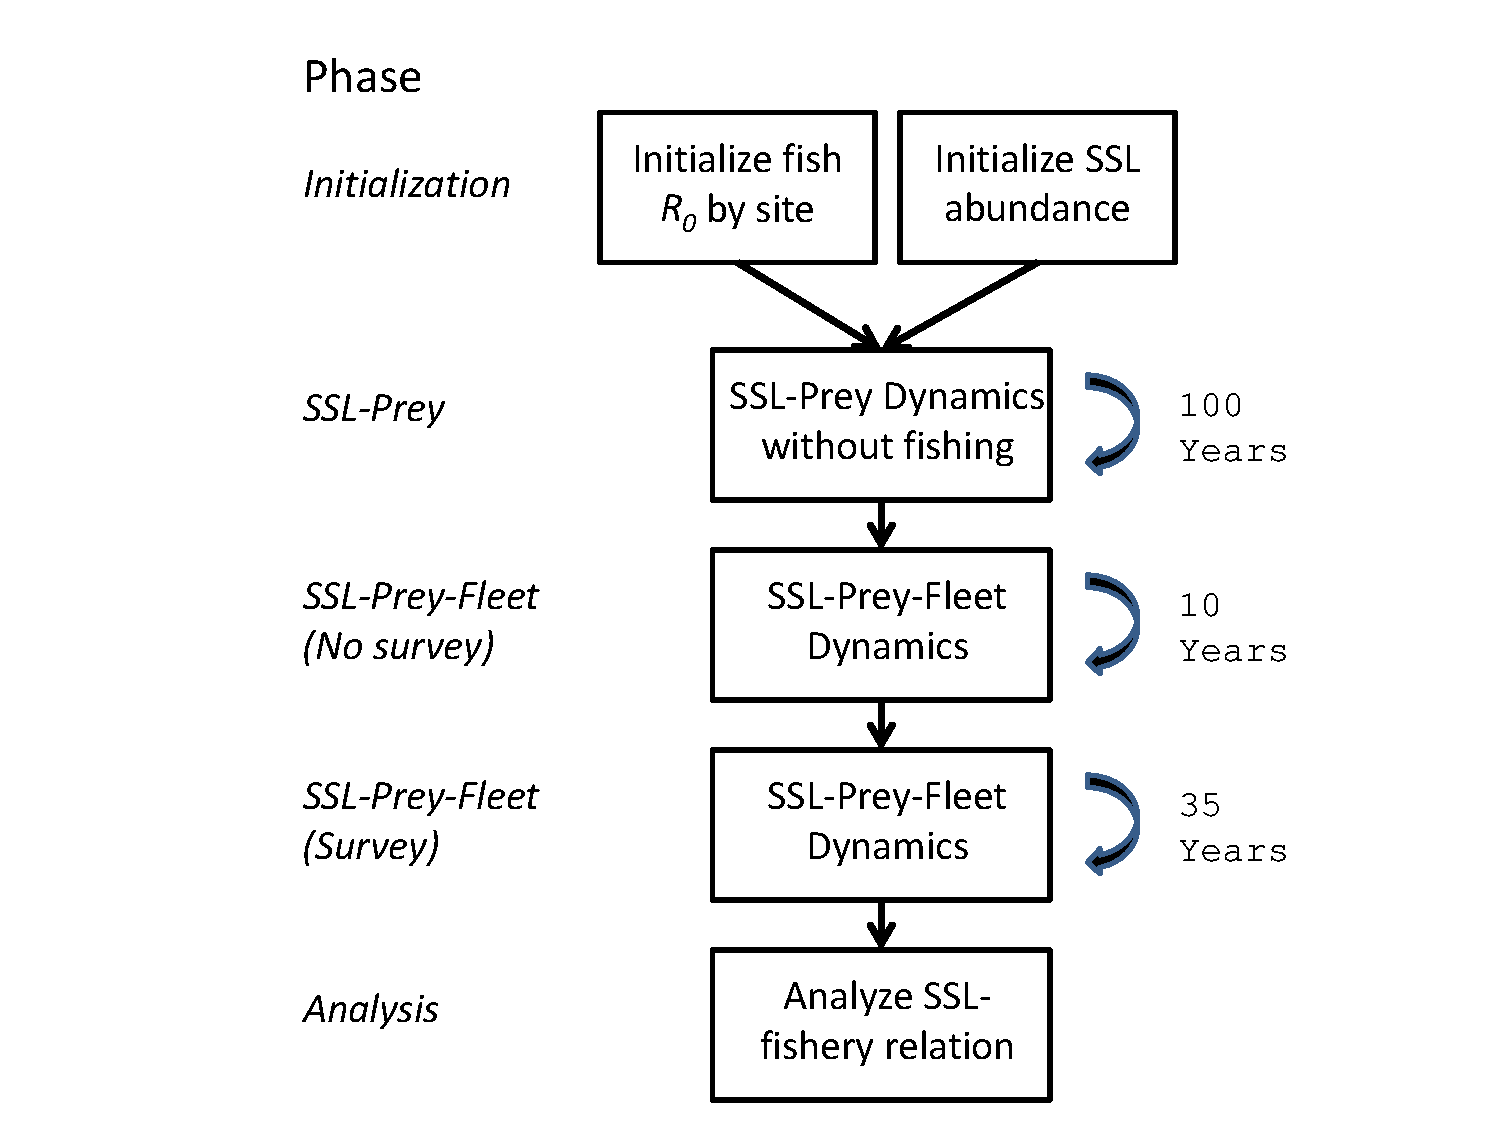
\includegraphics[width= \textwidth]{sim_diagram.pdf}
\end{center}
\caption{A depiction of the simulation structure used in analysis of Stellar sea lion (SSL) and fishery
 variables.  At the beginning of each simulation, predator (SSL) and prey (fish) populations are initialized at stable age distributions. After 100 years of simulating predator-prey dynamics to equalize numbers and induce variability in age structure due to fish recruitment stochasticity, fishing is introduced.  Following 10 years of fishing with no survey, simulated aerial surveys are assumed to occur for the next 35 years (at which time catch and CPUE are also calculated).  Finally, after simulated time series are gathered, data are analyzed via generalized linear mixed models to summarize relationships between SSL and fishing variables.}
\label{fig:sim_diagram}
\end{figure}


\end{document}
